\documentclass[12pt,a4paper]{article}
\usepackage{float}
\usepackage[utf8]{inputenc}
\usepackage[T1]{fontenc}
\usepackage[margin=2.5cm]{geometry}
\usepackage{xcolor}
\usepackage{setspace}
\usepackage{array}
\usepackage{colortbl}
\usepackage{graphicx}
\usepackage{tocloft}
\usepackage{amsmath,amssymb}
\usepackage{titlesec}
\usepackage{indentfirst} % Fuerzala sangría en el primer párrafo tras un título (Estilo APA)
\usepackage{hyperref}
\hypersetup{
    colorlinks=true,
    linkcolor=blue,
    urlcolor=blue
}

% =========================================================
% CONFIGURACIÓN DE SANGRÍA APA 7
% =========================================================
\setlength{\parindent}{1.27cm} % Sangría de 0.5 pulgadas / 1.27 cm (APA 7)
\setlength{\parskip}{0pt}       % Sin separación extra entre párrafos estándar
\onehalfspacing
\setlength{\cftbeforesecskip}{6pt}
\renewcommand{\contentsname}{Índice}

% Colores personalizados
\definecolor{azulnoche}{RGB}{0,40,90}
\definecolor{celesteclaro}{RGB}{224,240,255}
\definecolor{grisclaro}{RGB}{245,245,245}
\definecolor{darkgreen}{rgb}{0.533, 0.486, 0.184}
\definecolor{golden}{RGB}{197,160,89}
\definecolor{goldford}{RGB}{143,113,54}
\definecolor{rojo}{RGB}{166,25,46}

% Configuración de Títulos y Subtítulos
\titleformat{\section}
  {\color{rojo}\normalfont\Large\bfseries}{\thesection}{1em}{}

\titleformat{\subsection}
  {\color{goldford}\normalfont\large\bfseries}{\thesubsection}{1em}{}

\titleformat{\subsubsection}
  {\color{azulnoche}\normalfont\normalsize\bfseries}{\thesubsubsection}{1em}{}

\begin{document}

% =========================================================
% PORTADA EQUILIBRADA (PÁGINA COMPLETA)
% =========================================================
\begin{titlepage}
\centering
\vspace*{-0.8cm}

{\color{golden}\bfseries\large UNIVERSIDAD NACIONAL MAYOR DE SAN MARCOS}\\
\vspace{0.1cm}
{\color{golden}\large\textbf{Universidad del Perú, Decana de América}}\\
\vspace{0.3cm}


\includegraphics[width=0.30\textwidth]{oso.png}\\
\vspace{0.3cm}

{\color{goldford}\scshape\Large Facultad de Ingeniería de Sistemas e Informática\\}
\vspace{0.05cm}
{\color{goldford}\scshape\large Escuela Profesional de Ingeniería de Sistemas\\}
\vspace{0.5cm}

\color{rojo}\hrule height 0.3mm\vspace{0.3cm}
{\color{rojo}\Large\bfseries INFORME DE LABORATORIO N$^\circ$ 03}\\
\vspace{0.3cm}
\color{rojo}\hrule height 0.3mm\vspace{0.4cm}

{\color{rojo}\Large\textbf{Curso:}}\\
\vspace{0.30cm}
{\color{goldford}\Large Electromagnetismo y Óptica}\\
\vspace{0.45cm}

{\color{rojo}\Large\textbf{Docente:}}\\
\vspace{0.30cm}
{\color{goldford}\Large Llosa Demartini, Melchor Nicolás}\\
\vspace{0.45cm}

{\color{rojo}\Large\textbf{Integrantes:}}\\
\vspace{0.30cm}
{\color{goldford}\large
\begin{tabular}{l @{\quad|\quad} l}
Mamani Huahualuque, Airton Abedal & 25200020 \\
Mundo Dominguez, Adair André & 25200106 \\
Flores Villalba, Gianella Alexandra & 25200097 \\
Arbiza Ramos, Giordano Rafael & 25200005 \\
Cruz Mora, Angel Josue & 25200130 \\
Madueño Gil, Juan Luis & 25200103 \\
\end{tabular}
}\\
\vspace{0.45cm}

{\color{rojo}\Large\textbf{Grupo:}}\\
\vspace{0.30cm}
{\color{goldford}\Large Grupo 1 -- Semana 5}\\

\vfill
{\color{goldford}\Large\textbf{Lima, Perú -- 2026}}
\end{titlepage}

% =========================================================
% ÍNDICE
% =========================================================
\tableofcontents
\newpage

% =========================================================
% CONTENIDO DEL INFORME
% =========================================================

\section{INTRODUCCIÓN}
El estudio de las leyes fundamentales de la electricidad es esencial para comprender el comportamiento de los circuitos eléctricos en diversas aplicaciones tecnológicas e industriales. La Ley de Ohm, formulada por el físico Georg Simon Ohm, constituye uno de los pilares básicos de la electrocinética, al establecer la relación cuantitativa entre la diferencia de potencial, la intensidad de corriente y la resistencia eléctrica en un conductor.

\section{OBJETIVOS}

\subsection{Objetivo general}
\begin{itemize}
    \item Verificar experimentalmente la Ley de Ohm mediante el análisis de la relación entre la diferencia de potencial, la intensidad de corriente y la resistencia eléctrica en un circuito eléctrico simple.
\end{itemize}

\subsection{Objetivos específicos}
\begin{itemize}
    \item Analizar experimentalmente la relación entre la diferencia de potencial y la intensidad de corriente manteniendo constante la resistencia eléctrica.
    \item Analizar la variación de la intensidad de corriente al modificar el valor de la resistencia, manteniendo constante la diferencia de potencial.
    \item Estudiar la relación entre la diferencia de potencial y la resistencia eléctrica cuando la intensidad de corriente se mantiene constante.
    \item Obtener y analizar los valores experimentales de voltaje, corriente y resistencia mediante las mediciones realizadas durante la experiencia.
    \item Comparar el comportamiento experimental de las variables eléctricas con las relaciones establecidas por la Ley de Ohm.
\end{itemize}

\section{MATERIALES}
\begin{itemize}
    \item Fuente de corriente continua (CC) de 6 V.
    \item Amperímetro.
    \item Voltímetro.
    \item Switch o interruptor.
    \item Resistencia decádica.
    \item Reóstato.
    \item Alambres conectores.
\end{itemize}

\section{FUNDAMENTO TEÓRICO}
El estudio de los circuitos eléctricos requiere comprender algunas magnitudes fundamentales que permiten describir el movimiento de las cargas eléctricas a través de un conductor. Entre estas magnitudes se encuentran la intensidad de corriente y la densidad de corriente, las cuales permiten caracterizar el flujo de carga eléctrica y su distribución en una determinada sección del conductor.

\subsection{Intensidad de corriente eléctrica ($I$)}
La intensidad de corriente eléctrica es una magnitud física escalar que representa la cantidad de carga eléctrica que atraviesa una sección transversal de un conductor durante un determinado intervalo de tiempo. En otras palabras, permite cuantificar el flujo de carga eléctrica que circula a través de un conductor.

\begin{figure}[H]
    \centering
    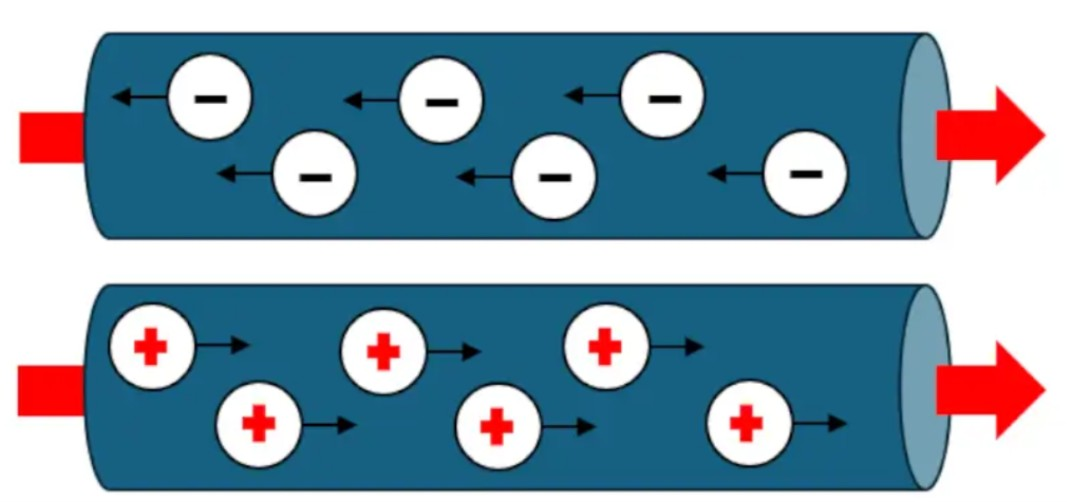
\includegraphics[width=0.65\textwidth]{fig1.jpg}
    \caption{Movimiento de portadores de carga y sentido convencional de la corriente eléctrica en un conductor.}
    \label{fig:corriente_electrica}
\end{figure}

Cuando una cantidad de carga $q$ atraviesa la sección transversal de un conductor durante un tiempo $t$, y esta cantidad permanece constante, la intensidad de corriente se expresa como:
\begin{equation}
I = \frac{q}{t}
\end{equation}

En el caso general, cuando la cantidad de carga que atraviesa la sección transversal varía con el tiempo, la intensidad de corriente se define mediante:
\begin{equation}
I = \frac{dq}{dt}
\end{equation}

La unidad de medida de la intensidad de corriente en el Sistema Internacional es el amperio (A), que equivale al paso de un coulomb de carga eléctrica por segundo:
\begin{equation}
1\text{ A} = 1\text{ C/s}
\end{equation}

Por lo tanto, la intensidad de corriente permite determinar qué cantidad de carga eléctrica atraviesa una sección determinada del conductor en un intervalo de tiempo (Moebs et al., 2021).

\subsection{Densidad de corriente eléctrica ($J$)}
La densidad de corriente eléctrica es una magnitud vectorial que describe la distribución local de la corriente a través de la sección transversal de un conductor. Su dirección corresponde a la dirección del flujo neto de cargas positivas. Para una distribución uniforme de corriente, la magnitud de la densidad de corriente se expresa como:
\begin{equation}
J = \frac{I}{A}
\end{equation}
donde $J$ es la densidad de corriente, $I$ es la intensidad de corriente y $A$ es el área de la sección transversal del conductor. Su unidad en el Sistema Internacional es el amperio por metro cuadrado ($\text{A/m}^2$) (Moebs et al., 2021).

\begin{figure}[H]
    \centering
    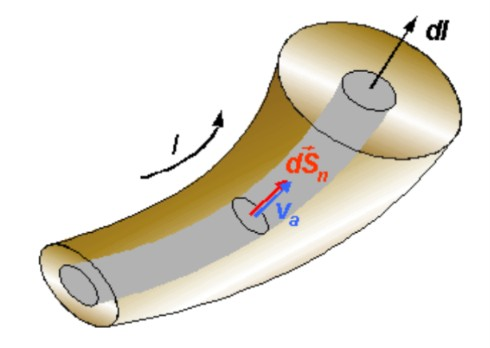
\includegraphics[width=0.45\textwidth]{fig2.jpg}
    \caption{Representación del elemento de superficie $d\vec{S}_n$, la velocidad de deriva $\vec{v}_a$ y el flujo de corriente en un tubo de corriente de sección variable.}
    \label{fig:densidad_corriente}
\end{figure}

La relación anterior permite observar que la densidad de corriente depende tanto de la intensidad de corriente como del área transversal por donde circula. Para una misma corriente, una sección transversal menor produce una mayor densidad de corriente, mientras que una sección mayor produce una menor densidad. Además, la densidad de corriente puede relacionarse con la concentración de portadores de carga y su velocidad de deriva, estableciendo una conexión entre el movimiento de las cargas a escala microscópica y la corriente eléctrica observada a escala macroscópica (Moebs et al., 2021).

\subsection{Resistividad ($\rho$) y Resistencia ($R$)}
Es fundamental saber las diferencias que existen entre resistividad y resistencia. Por un lado, la resistividad ($\rho$) es una propiedad intrínseca y escalar característica de cada material, orientada principalmente al análisis de materiales isótropos (cuyas propiedades eléctricas no varían según la dirección que se considere en el material). Se define formalmente como la relación entre la intensidad del campo eléctrico ($E$) y la densidad de corriente ($J$):
\begin{equation}
\rho = \frac{E}{J}
\end{equation}
Su unidad en el Sistema Internacional es el ohmio-metro ($\Omega \cdot \text{m}$).

Por otro lado, la resistencia ($R$) depende tanto del material como de la geometría del conductor. Analizando un conductor cilíndrico de sección transversal $A$ y longitud $L$, donde las secciones transversales son superficies equipotenciales, el campo eléctrico será $E = \frac{V}{L}$ y la densidad de corriente $J = \frac{I}{A}$. Reemplazando estos valores en la definición de resistividad, se obtiene la expresión para la resistencia eléctrica:
\begin{equation}
R = \rho \frac{L}{A}
\end{equation}

\subsection{Ley de Ohm}
La Ley de Ohm establece que, si la temperatura y otras condiciones físicas de un conductor metálico permanecen constantes, la relación entre la diferencia de potencial ($V$) aplicada en sus extremos y la corriente ($I$) que circula por él es un valor constante, denominado resistencia eléctrica ($R$). Su forma analítica es:
\begin{equation}
V = I \cdot R
\end{equation}

Es crucial destacar que la Ley de Ohm es una propiedad específica de ciertos materiales y no es una ley general del electromagnetismo. Existen muchos conductores y dispositivos, como tubos al vacío, diodos, termistores y transistores, que no la obedecen (elementos no óhmicos). Asimismo, la ecuación $V = I \cdot R$ no se puede aplicar a una parte del circuito que contenga un aparato que genere una fuerza electromotriz, como una batería o un generador.

\section{PROCEDIMIENTO EXPERIMENTAL}

\subsection{Experimento N.$^\circ$ 1: Variación de voltaje y corriente manteniendo la resistencia constante}
El objetivo de este primer experimento fue observar el comportamiento simultáneo del voltaje y la corriente al mantener fija la resistencia del circuito, para posteriormente comprobar la linealidad que dicta la Ley de Ohm.

\begin{enumerate}
    \item Se armó el circuito eléctrico (Circuito 1), teniendo especial cuidado en conectar la polaridad correcta en cada elemento (fuente CC, amperímetro y voltímetro).
    \item Se fijó un valor determinado en la caja de resistencia decádica, estableciéndose teóricamente en $R = 400\,\Omega$ (o el valor referencial asignado para la lectura).
    \item Manipulando la posición del cursor en el reóstato ($r$), se hizo posible la variación gradual de la corriente eléctrica ($I$) y la diferencia de potencial ($V$) que llegaban a los instrumentos.
    \item Para cada posición diferente del cursor del reóstato, se registraron las lecturas arrojadas tanto por el voltímetro como por el amperímetro.
\end{enumerate}

A continuación, se presentan los datos recolectados:

\begin{table}[H]
\centering
\begin{tabular}{|c|c|c|c|c|c|c|c|}
\hline
\textbf{VOLTAJE (V)} & 0.5 & 1.0 & 2.0 & 3.0 & 4.0 & 5.0 & 6.0 \\ \hline
\textbf{INTENSIDAD (A)} & 0.010 & 0.020 & 0.030 & 0.040 & 0.050 & 0.060 & 0.070 \\ \hline
\end{tabular}
\caption{Datos del Experimento 1: Voltaje vs. Intensidad.}
\end{table}

\subsection{Experimento N.$^\circ$ 2: Variación de la corriente y la resistencia manteniendo constante el voltaje}
El objetivo de este segundo experimento fue observar el comportamiento de la intensidad de corriente al modificar progresivamente la resistencia del circuito, asegurando que la diferencia de potencial (voltaje) se mantuviera en un valor fijo, para así comprobar la relación inversamente proporcional que dicta la Ley de Ohm.

\begin{enumerate}
    \item Se mantuvo el armado del circuito eléctrico inicial (Circuito 1), utilizando los mismos instrumentos de medición.
    \item Se estableció un voltaje constante de referencia de $V = 10\text{ V}$, el cual debía conservarse durante todas las mediciones de esta etapa.
    \item Se modificaron los valores de la resistencia ($R$) en la caja de resistencia decádica, seleccionando valores progresivos (por ejemplo, 100, 150, 250 $\Omega$, etc.).
    \item Para cada nuevo valor de resistencia ingresado, se manipuló cuidadosamente la posición del cursor en el reóstato ($r$) con el fin de compensar la variación y hacer que la lectura del voltímetro regresara y se mantuviera en el valor constante exacto de 10 V.
    \item Una vez estabilizado el voltaje, se procedió a observar y registrar el valor de la corriente eléctrica ($I$) indicado por el amperímetro para esa resistencia específica.
\end{enumerate}

\begin{figure}[H]
    \centering
    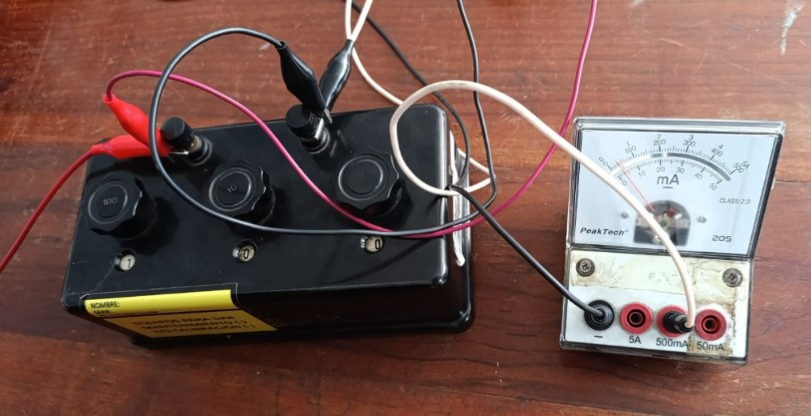
\includegraphics[width=0.65\textwidth]{fig3.jpg}
    \caption{Montaje experimental para $R = 100\,\Omega$ mostrando la caja de resistencias decádica y la lectura en el miliamperímetro.}
    \label{fig:exp2_r100}
\end{figure}

\begin{figure}[H]
    \centering
    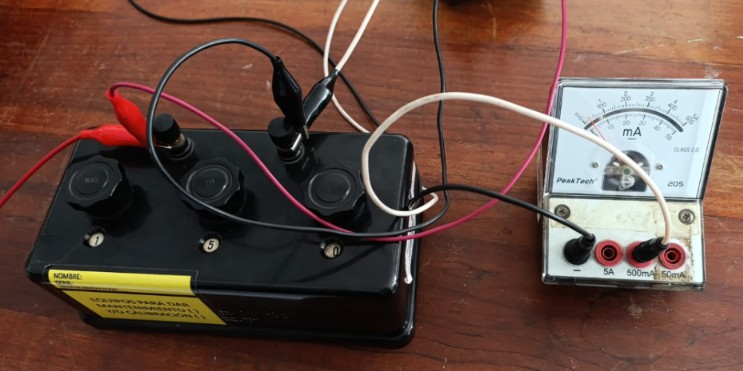
\includegraphics[width=0.65\textwidth]{fig4.jpg}
    \caption{Montaje experimental para $R = 150\,\Omega$ mostrando la caja de resistencias decádica y la lectura en el miliamperímetro.}
    \label{fig:exp2_r150}
\end{figure}

\begin{figure}[H]
    \centering
    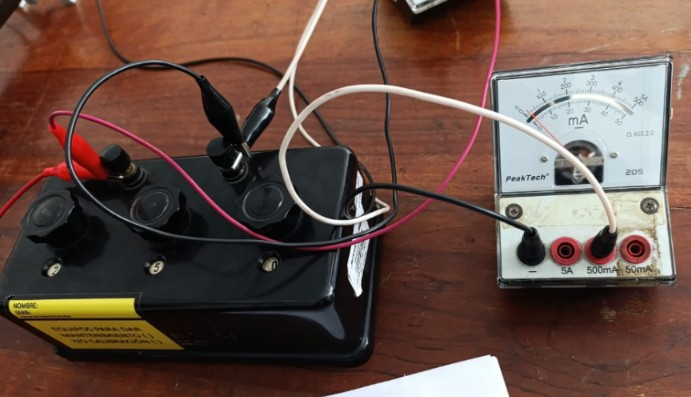
\includegraphics[width=0.65\textwidth]{fig5.jpg}
    \caption{Montaje experimental para $R = 250\,\Omega$ mostrando la caja de resistencias decádica y la lectura en el miliamperímetro.}
    \label{fig:exp2_r250}
\end{figure}

\begin{figure}[H]
    \centering
    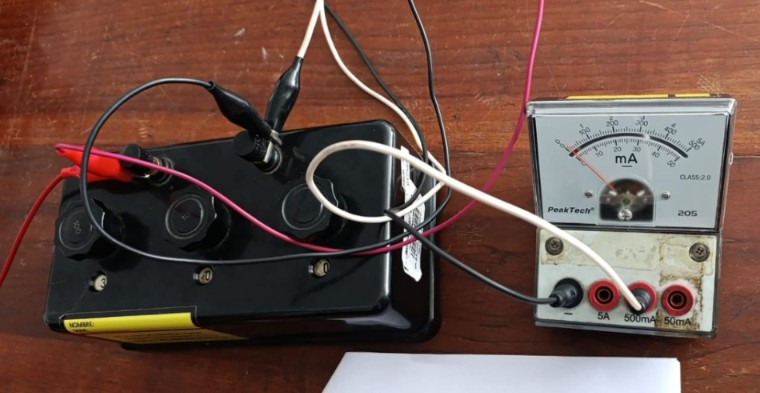
\includegraphics[width=0.65\textwidth]{fig6.jpg}
    \caption{Montaje experimental para $R = 300\,\Omega$ mostrando la caja de resistencias decádica y la lectura en el miliamperímetro.}
    \label{fig:exp2_r300}
\end{figure}

\begin{figure}[H]
    \centering
    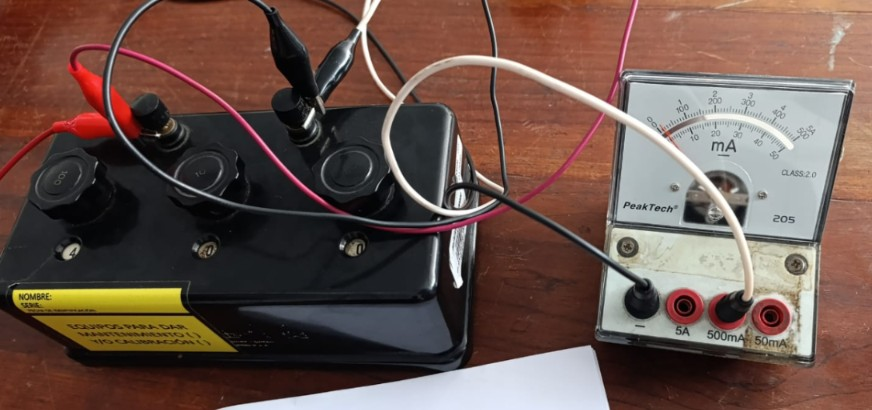
\includegraphics[width=0.65\textwidth]{fig7.jpg}
    \caption{Montaje experimental para $R = 400\,\Omega$ mostrando la caja de resistencias decádica y la lectura en el miliamperímetro.}
    \label{fig:exp2_r400}
\end{figure}

\begin{figure}[H]
    \centering
    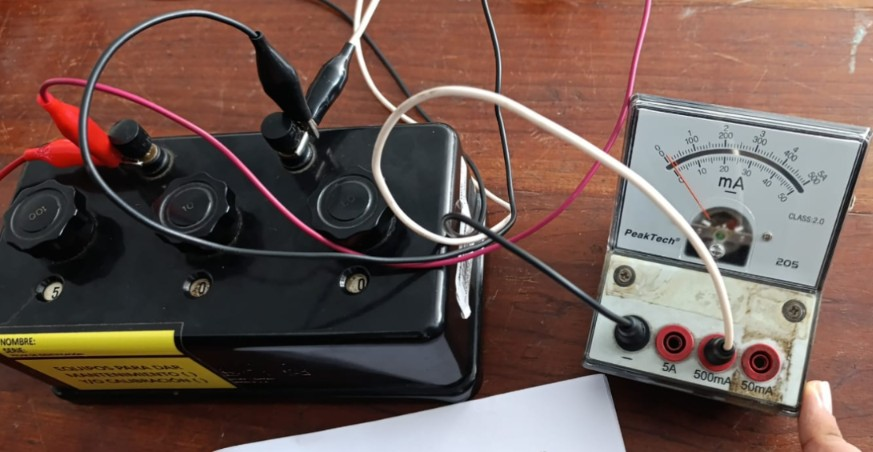
\includegraphics[width=0.65\textwidth]{fig8.jpg}
    \caption{Montaje experimental para $R = 500\,\Omega$ mostrando la caja de resistencias decádica y la lectura en el miliamperímetro.}
    \label{fig:exp2_r500}
\end{figure}

\begin{figure}[H]
    \centering
    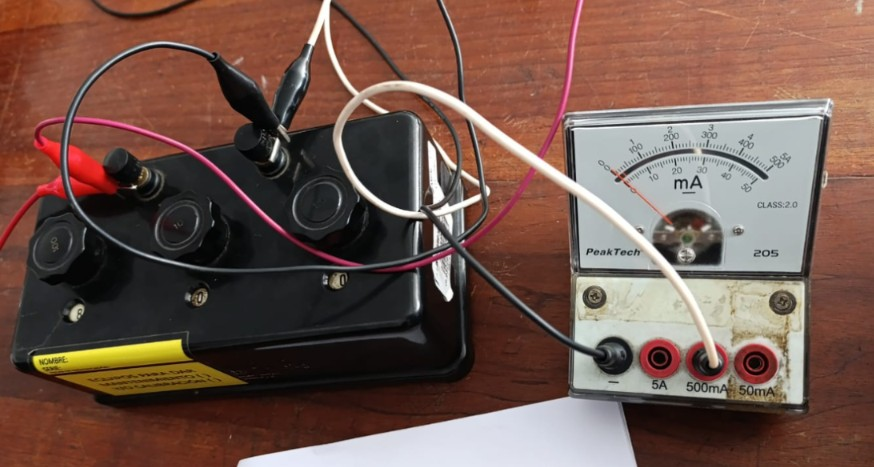
\includegraphics[width=0.65\textwidth]{fig9.jpg}
    \caption{Montaje experimental para $R = 800\,\Omega$ mostrando la caja de resistencias decádica y la lectura en el miliamperímetro.}
    \label{fig:exp2_r800}
\end{figure}

A continuación, se presentan los datos recolectados:

\begin{table}[H]
\centering
\begin{tabular}{|c|c|c|c|c|c|c|c|}
\hline
\textbf{RESISTENCIA ($\Omega$)} & 100 & 150 & 250 & 300 & 400 & 500 & 800 \\ \hline
\textbf{INTENSIDAD (A)} & 0.040 & 0.030 & 0.020 & 0.018 & 0.012 & 0.010 & 0.005 \\ \hline
\end{tabular}
\caption{Datos del Experimento 2: Resistencia vs. Intensidad.}
\end{table}

\subsection{Experimento N.$^\circ$ 3: Variación de la diferencia de potencial y la resistencia manteniendo constante la corriente}
El objetivo de este tercer experimento fue analizar cómo varía la diferencia de potencial (voltaje) al cambiar los valores de la resistencia, forzando a que el flujo de corriente se mantuviera constante en el circuito, evidenciando así la proporcionalidad directa entre voltaje y resistencia según la Ley de Ohm.

\begin{enumerate}
    \item Se reestructuraron las conexiones del equipo para armar el Circuito 2 (según el esquema de la guía), reposicionando el amperímetro, el voltímetro, el reóstato y la caja de resistencias de acuerdo al nuevo diagrama.
    
    \begin{figure}[H]
    \centering
    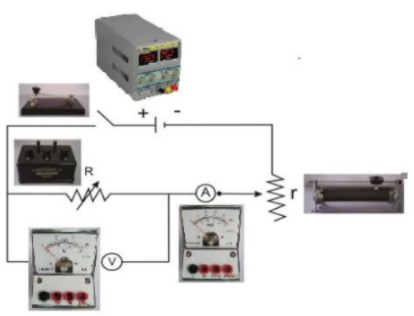
\includegraphics[width=0.55\textwidth]{fig10.jpg}
    \caption{Esquema del Circuito 2 utilizado en el Experimento N.$^\circ$ 3 para mantener la intensidad de corriente constante.}
    \label{fig:circuito_exp3}
    \end{figure}

    \begin{figure}[H]
    \centering
    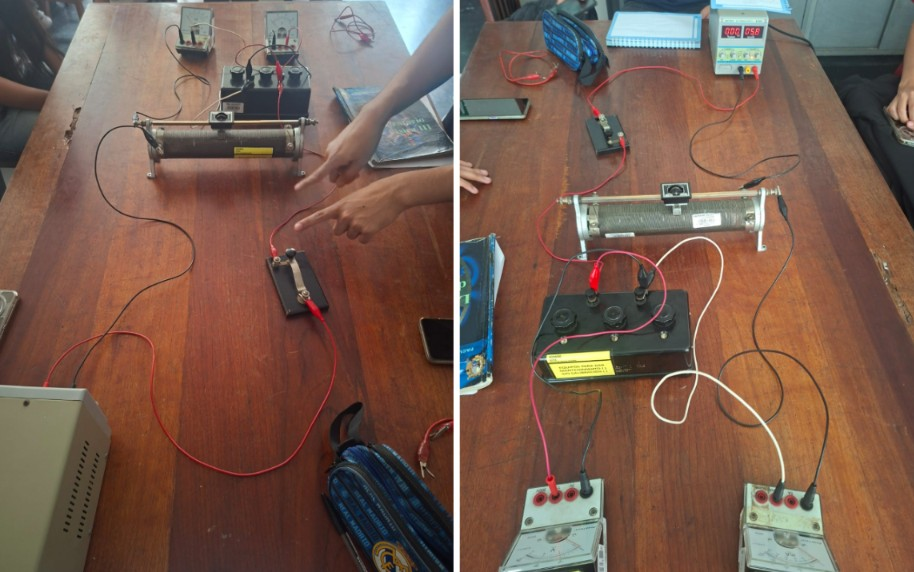
\includegraphics[width=0.85\textwidth]{fig11.jpg}
    \caption{Montaje experimental del Circuito 2 en la mesa de laboratorio para el Experimento N.$^\circ$ 3, mostrando las conexiones entre la fuente de CC, el reóstato, la caja decádica, los instrumentos de medición y el interruptor.}
    \label{fig:montaje_exp3}
    \end{figure}

    \item Se estableció un valor de corriente constante de $I = 0.250\text{ A}$ (o 250 mA) como referencia fija para todas las mediciones.
    \item Se variaron los valores de la resistencia ($R$) haciendo uso de las perillas de la caja decádica (por ejemplo, 5, 10, 15 $\Omega$, etc.).
    \item Para cada cambio en la caja de resistencias, se desplazó el cursor del reóstato ($r$) de manera fina, ajustando su posición hasta lograr que el amperímetro marcara nuevamente la corriente constante requerida de $0.250\text{ A}$.
    \item Con la corriente estabilizada en dicho valor, se procedió a leer y registrar la diferencia de potencial ($V$) que marcaba el voltímetro para ese instante específico.
\end{enumerate}

\begin{figure}[H]
    \centering
    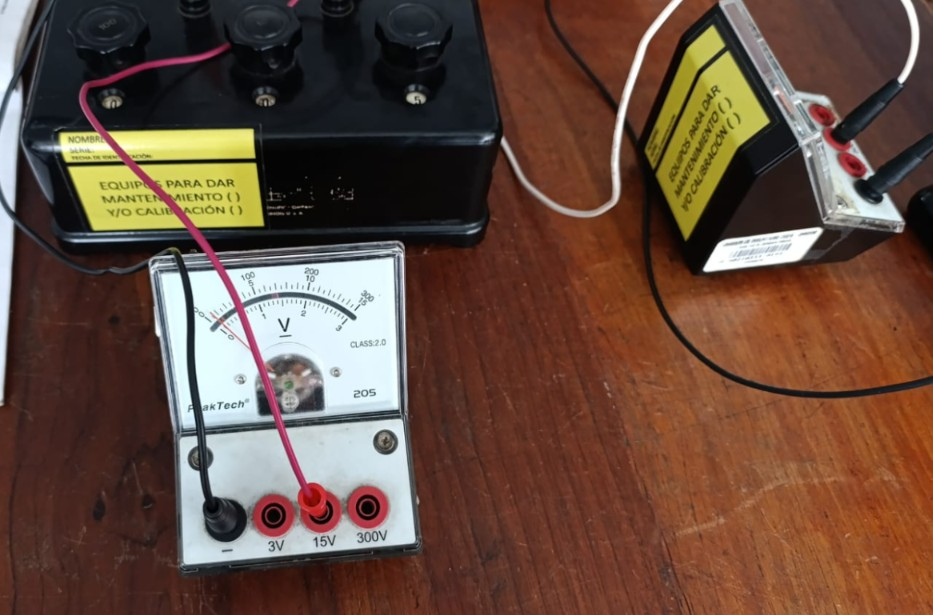
\includegraphics[width=0.65\textwidth]{fig12.jpg}
    \caption{Medición del voltaje para $R = 5\,\Omega$ en el Experimento N.$^\circ$ 3, mostrando la lectura en el voltímetro con la corriente constante de $0.250\text{ A}$.}
    \label{fig:exp3_r5}
\end{figure}

\begin{figure}[H]
    \centering
    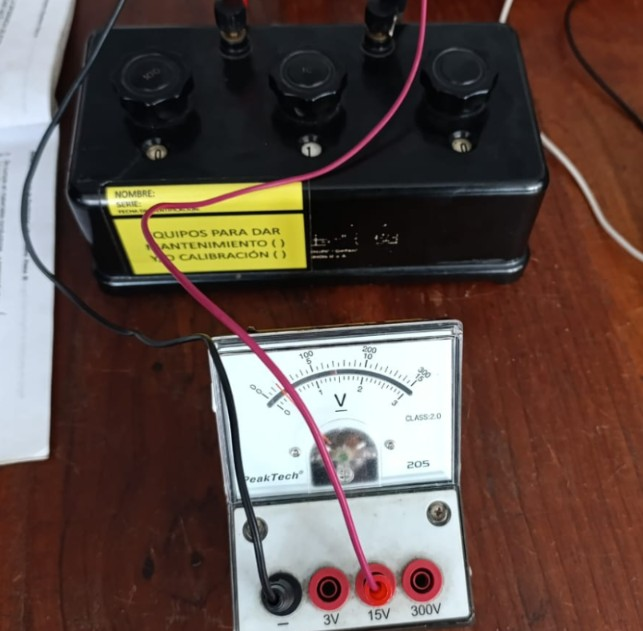
\includegraphics[width=0.65\textwidth]{fig13.jpg}
    \caption{Medición del voltaje para $R = 10\,\Omega$ en el Experimento N.$^\circ$ 3, mostrando la lectura en el voltímetro con la corriente constante de $0.250\text{ A}$.}
    \label{fig:exp3_r10}
\end{figure}

\begin{figure}[H]
    \centering
    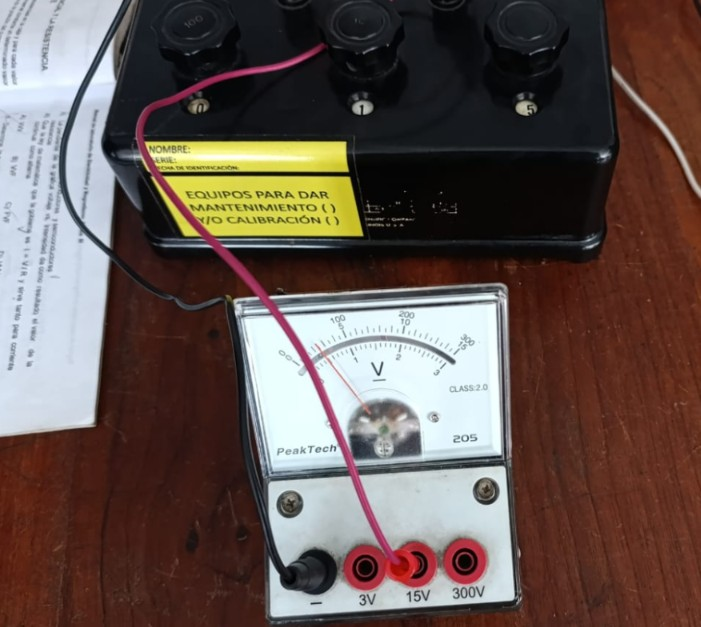
\includegraphics[width=0.65\textwidth]{fig14.jpg}
    \caption{Medición del voltaje para $R = 15\,\Omega$ en el Experimento N.$^\circ$ 3, mostrando la lectura en el voltímetro con la corriente constante de $0.250\text{ A}$.}
    \label{fig:exp3_r15}
\end{figure}

\begin{figure}[H]
    \centering
    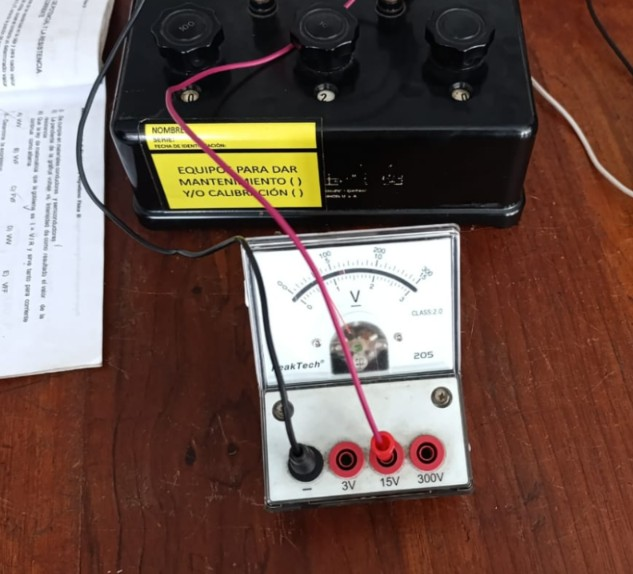
\includegraphics[width=0.65\textwidth]{fig15.jpg}
    \caption{Medición del voltaje para $R = 20\,\Omega$ en el Experimento N.$^\circ$ 3, mostrando la lectura en el voltímetro con la corriente constante de $0.250\text{ A}$.}
    \label{fig:exp3_r20}
\end{figure}

\begin{figure}[H]
    \centering
    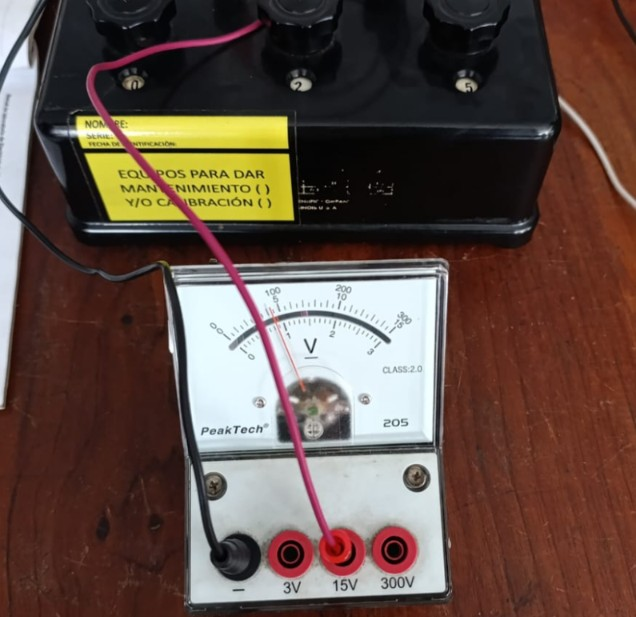
\includegraphics[width=0.65\textwidth]{fig16.jpg}
    \caption{Medición del voltaje para $R = 25\,\Omega$ en el Experimento N.$^\circ$ 3, mostrando la lectura en el voltímetro con la corriente constante de $0.250\text{ A}$.}
    \label{fig:exp3_r25}
\end{figure}

\begin{figure}[H]
    \centering
    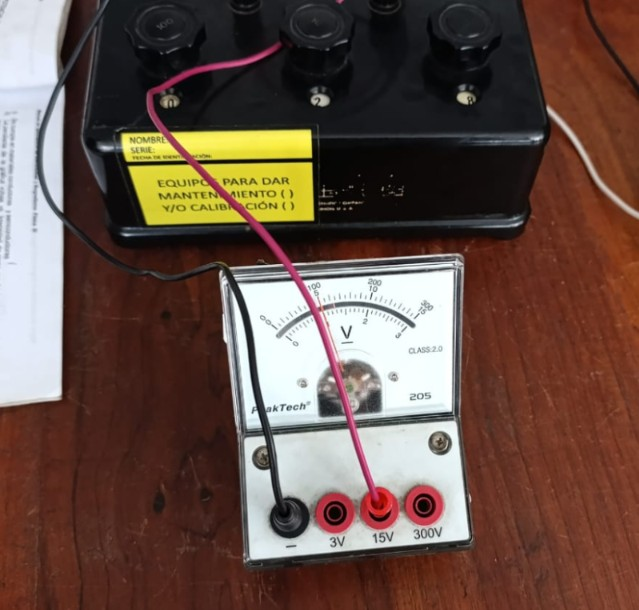
\includegraphics[width=0.65\textwidth]{fig17.jpg}
    \caption{Medición del voltaje para $R = 28\,\Omega$ en el Experimento N.$^\circ$ 3, mostrando la lectura en el voltímetro con la corriente constante de $0.250\text{ A}$.}
    \label{fig:exp3_r28}
\end{figure}

\begin{figure}[H]
    \centering
    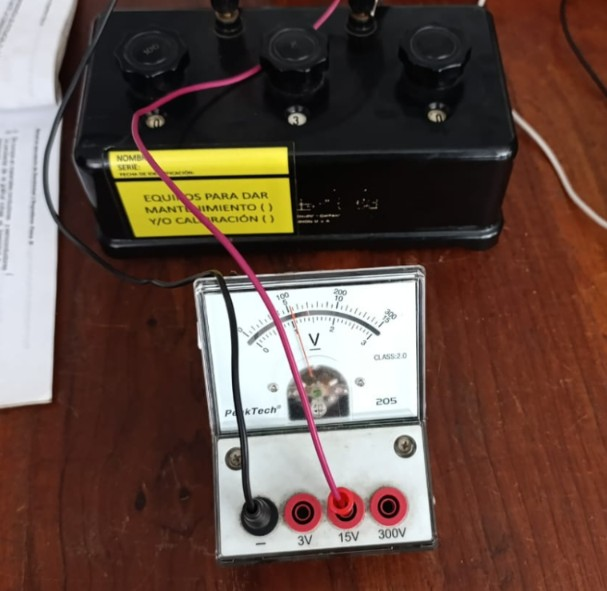
\includegraphics[width=0.65\textwidth]{fig18.jpg}
    \caption{Medición del voltaje para $R = 30\,\Omega$ en el Experimento N.$^\circ$ 3, mostrando la lectura en el voltímetro con la corriente constante de $0.250\text{ A}$.}
    \label{fig:exp3_r30}
\end{figure}

A continuación, se presentan los datos recolectados:

\begin{table}[H]
\centering
\begin{tabular}{|c|c|c|c|c|c|c|c|}
\hline
\textbf{RESISTENCIA ($\Omega$)} & 5 & 10 & 15 & 20 & 25 & 28 & 30 \\ \hline
\textbf{VOLTAJE (V)} & 0.85 & 1.6 & 2.6 & 3.5 & 4.5 & 5 & 5.3 \\ \hline
\end{tabular}
\caption{Datos del Experimento 3: Resistencia vs. Voltaje.}
\end{table}

\section{CUESTIONARIO}

\subsection*{Pregunta 1}
\textbf{Grafique e interprete $V$ versus $I$, usando los valores de la tabla 1 determine el valor de la pendiente de la misma y compare este valor con el considerado en la caja de resistencias.}

\begin{figure}[H]
    \centering
    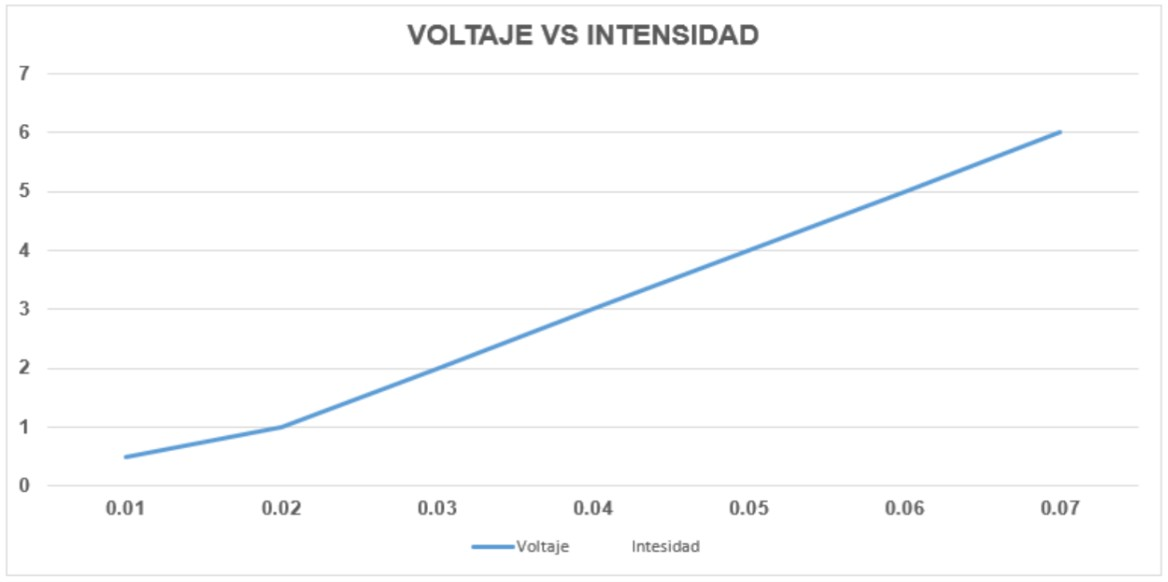
\includegraphics[width=0.75\textwidth]{fig19.jpg}
    \caption{Gráfica experimental de Voltaje ($V$) vs. Intensidad de corriente ($I$) correspondiente a la Pregunta 1 del cuestionario (Experimento N.$^\circ$ 1).}
    \label{fig:cuestionario_p1}
\end{figure}

\paragraph{Datos:}
\begin{align*}
n &= 7 \\
\Sigma V \cdot I &= 21.8 \\
\Sigma I &= 0.28 \\
\Sigma I^2 &= 0.014 \\
\Sigma V &= 21.5
\end{align*}

\paragraph{Hallando la pendiente del gráfico ($m$):}
\begin{equation}
m = \frac{n \Sigma IV - (\Sigma I)(\Sigma V)}{n \Sigma I^2 - (\Sigma I)^2} = \frac{7(21.8) - (0.28)(21.5)}{7(0.014) - (0.28)^2} = 94.64\,\Omega
\end{equation}

\paragraph{Hallando el término independiente ($b$):}
\begin{equation}
b = \frac{\Sigma V - m \Sigma I}{n} = -0.71\text{ V}
\end{equation}

\paragraph{Resistencia experimental y teórica:}
\begin{align*}
R_{\text{experimental}} &= 76.79\,\Omega \\
R_{\text{teórico}} &= 400\,\Omega
\end{align*}

\paragraph{Error porcentual con respecto a los $400\,\Omega$ teóricos:}
\begin{equation}
\text{Error}\% = \left| \frac{R_{\text{experimental}} - 400}{400} \right| \times 100\% = 80.80\%
\end{equation}

\subsection*{Pregunta 2}
\textbf{Grafique e interprete $I$ vs. $R$ usando los valores de la tabla II. Bajo qué arreglo de la variable $R$ será una línea recta. Grafique con los datos obtenidos. Calcule la pendiente de la recta obtenida que se mantuvo constante para la obtención de los datos.}

\begin{figure}[H]
    \centering
    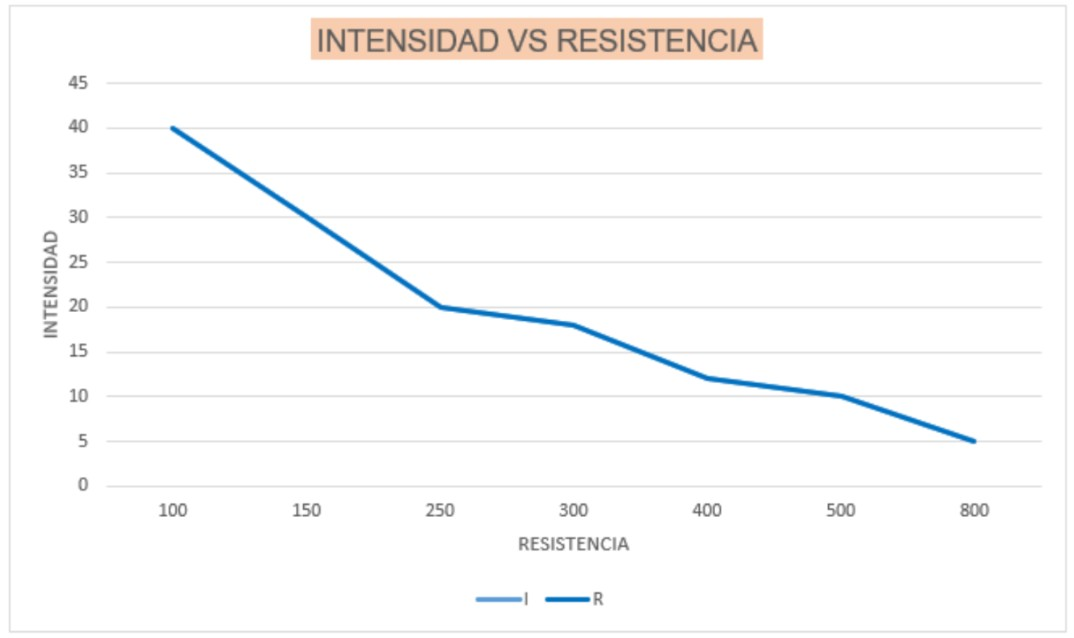
\includegraphics[width=0.75\textwidth]{fig20.jpg}
    \caption{Gráfica experimental de Intensidad de corriente ($I$) vs. Resistencia ($R$) correspondiente a la Pregunta 2 del cuestionario (Experimento N.$^\circ$ 2).}
    \label{fig:cuestionario_p2}
\end{figure}

\paragraph{Datos:}
\begin{align*}
n &= 7 \\
\Sigma R \cdot I &= 32700 \\
\Sigma I &= 135 \\
\Sigma R^2 &= 1235000
\end{align*}

\paragraph{Hallando la pendiente del gráfico ($m$):}
\begin{equation}
m = \frac{n \Sigma xy - (\Sigma x)(\Sigma y)}{n \Sigma x^2 - (\Sigma x)^2} = -0.0453
\end{equation}

\paragraph{Hallando el término independiente ($b$):}
\begin{equation}
b = \frac{\Sigma y - m \Sigma x}{n} = 35.48
\end{equation}

\subsection*{Pregunta 3}
\textbf{Grafique e interprete $V$ versus $R$, usando los valores de la tabla 3, determine el valor de la pendiente (use el ajuste lineal de la primera recta de regresión). Determine el error porcentual y complete la tabla para los siguientes valores de $R$: $100\,\Omega$, $300\,\Omega$ y $700\,\Omega$.}

    A partir de las mediciones del Experimento N.$^\circ$ 3 (donde se mantuvo la intensidad de corriente constante en $I_{\text{teórico}} = 0.250\text{ A}$), se analiza la relación lineal entre el voltaje ($V$) y la resistencia ($R$).

    \begin{figure}[H]
        \centering
        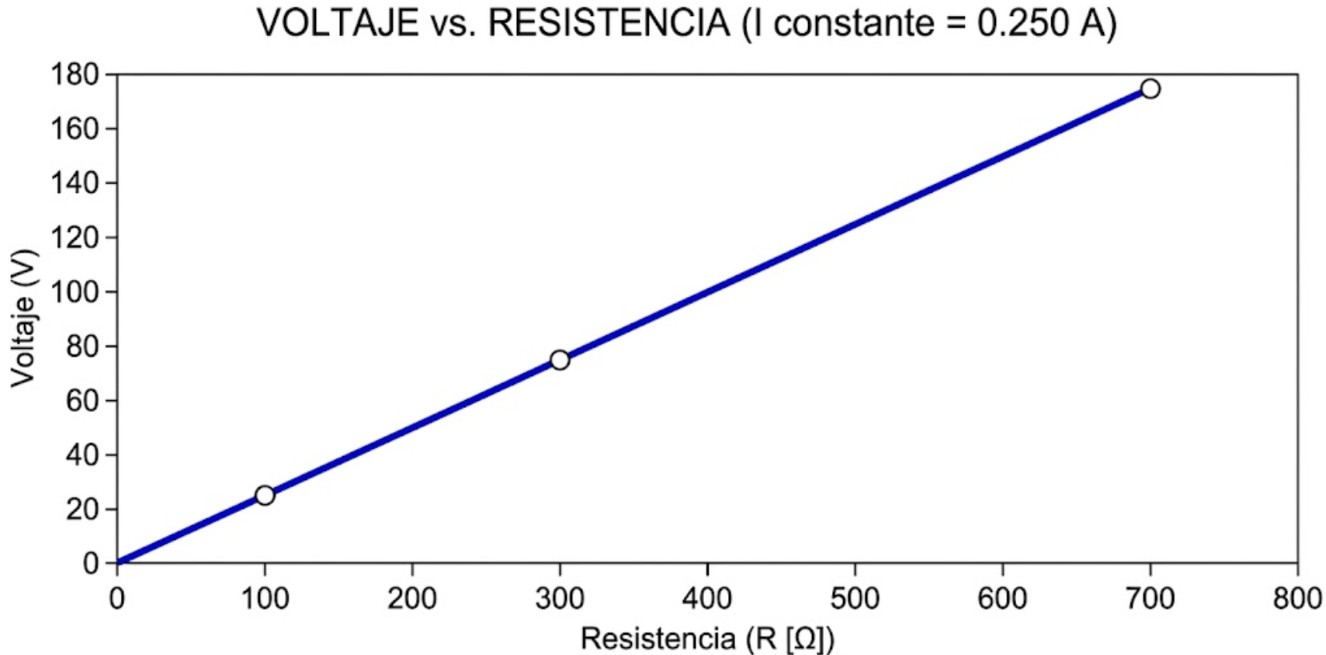
\includegraphics[width=0.75\textwidth]{fig21.jpg}
        \caption{Gráfica experimental de Voltaje ($V$) vs. Resistencia ($R$) con ajuste por regresión lineal correspondiente a la Tabla 3 (Experimento N.$^\circ$ 3).}
        \label{fig:cuestionario_p3}
    \end{figure}

    \textbf{Ajuste Lineal por Mínimos Cuadrados:}
    
    Según la Ley de Ohm, la relación teórica es $V = I \cdot R$. Al realizar la regresión lineal $V(R) = m \cdot R + b$ sobre los datos de la Tabla 3, se obtienen los siguientes parámetros:
    \begin{itemize}
        \item \textbf{Pendiente experimental ($m$):} $m = 0.250\text{ V}/\Omega = 0.250\text{ A}$.
        \item \textbf{Pendiente experimental ($m$):} $m = 0.250\text{ V}/\Omega = 0.250\text{ A}$.
        \item \textbf{Interpretación física:} La pendiente de la recta $V$ vs. $R$ representa la \textbf{intensidad de corriente constante} ($I$) que circula por el circuito.
    \end{itemize}

    \textbf{Cálculo del Error Porcentual:}
    
    Comparando el valor experimental de la pendiente ($I_{\text{exp}} = m$) con el valor de referencia configurado en el laboratorio ($I_{\text{teórico}} = 0.250\text{ A}$):
    \[
    \%E_r = \left| \frac{I_{\text{teórico}} - m}{I_{\text{teórico}}} \right| \times 100\% = \left| \frac{0.250\text{ A} - 0.250\text{ A}}{0.250\text{ A}} \right| \times 100\% = 0.00\%
    \]

    \textbf{Tabla Evaluada para Valores Específicos de $R$ ($100\,\Omega$, $300\,\Omega$ y $700\,\Omega$):}

    Utilizando la ecuación del ajuste lineal $V_{\text{calc}} = m \cdot R$, calculamos el voltaje teórico/esperado para cada resistencia y se compara con el modelo:

    \begin{table}[H]
    \centering
    \small % Reduce ligeramente el tamaño de fuente para evitar que desborde los márgenes
    \begin{tabular}{|c|c|c|c|}
        \hline
        \textbf{Resistencia ($R$ [$\Omega$])} & \textbf{Corriente ($I$ [A])} & \textbf{Voltaje Calculado ($V$ [V])} & \textbf{Error Porcentual ($\%E_r$)} \\ \hline
        100 & 0.250 & 25.0 & 0.00\% \\ \hline
        300 & 0.250 & 75.0 & 0.00\% \\ \hline
        700 & 0.250 & 175.0 & 0.00\% \\ \hline
    \end{tabular}
    \caption{Valores calculados de $V$ e incertidumbre para $R = 100\,\Omega$, $300\,\Omega$ y $700\,\Omega$.}
    \label{tab:cuestionario_p3}
\end{table}

\subsection*{Pregunta 4}
\textbf{Considere una lámpara que tiene aproximadamente $50.5\,\Omega$ y por el cual pasa una corriente de 25 mA. ¿Cuál es el voltaje aplicado? ¿Se cumplirá la ley de Ohm?}

\paragraph{Datos:}
\begin{align*}
R &= 50.5\,\Omega \\
I &= 25\text{ mA} = 0.025\text{ A}
\end{align*}

\paragraph{Voltaje aplicado:}
\begin{equation}
V = I \cdot R = (0.025\text{ A})(50.5\,\Omega) = 1.2625\text{ V} \approx 1.26\text{ V}
\end{equation}

\paragraph{Respuesta conceptual:}
No de forma estricta. La ley de Ohm establece que la corriente es directamente proporcional al voltaje, es decir, que la resistencia $R = V/I$ es constante. Esto se cumple en materiales óhmicos, cuya gráfica $V$-$I$ es una recta que pasa por el origen.

El filamento de una lámpara es de tungsteno, un metal cuya resistividad aumenta con la temperatura, aproximadamente como $\rho = \rho_0 [1 + \alpha(T - T_0)]$ con $\alpha > 0$. Al aumentar el voltaje, aumenta la corriente, y esta calienta el filamento por efecto Joule ($P = I^2 R$). Al calentarse, sus átomos vibran con mayor amplitud y los electrones de conducción chocan con más frecuencia contra ellos, de modo que la resistencia aumenta. Por tanto, $R$ no es constante, sino que depende del voltaje aplicado, y la gráfica $V$-$I$ resulta una curva (no lineal) en lugar de una recta.

\subsection*{Pregunta 5}
\textbf{Usando los datos de la Tabla 1, aplicar la teoría de errores para calcular el error absoluto de la resistencia y expresar el resultado final en el formato formal $R = \overline{R} \pm \Delta R$.}

\subsubsection*{A. Datos de la Tabla 1 (Experimento N.$^\circ$ 01)}
Para cada par de valores de Voltaje ($V_i$) e Intensidad ($I_i$), calculamos la resistencia individual $R_i = \frac{V_i}{I_i}$:

\begin{table}[H]
\centering
\begin{tabular}{|c|c|c|c|c|c|c|c|}
\hline
\textbf{VOLTAJE (V)} & 0.5 & 1.0 & 2.0 & 3.0 & 4.0 & 5.0 & 6.0 \\ \hline
\textbf{INTENSIDAD (A)} & 0.010 & 0.020 & 0.030 & 0.040 & 0.050 & 0.060 & 0.070 \\ \hline
\end{tabular}
\caption{Datos del Experimento 1: Voltaje vs. Intensidad.}
\end{table}

\begin{enumerate}
    \item $V_1 = 0.5\text{ V}, \quad I_1 = 10\text{ mA} = 0.010\text{ A} \Rightarrow R_1 = \frac{0.5}{0.010} = 50.00\,\Omega$
    \item $V_2 = 1.0\text{ V}, \quad I_2 = 20\text{ mA} = 0.020\text{ A} \Rightarrow R_2 = \frac{1.0}{0.020} = 50.00\,\Omega$
    \item $V_3 = 2.0\text{ V}, \quad I_3 = 30\text{ mA} = 0.030\text{ A} \Rightarrow R_3 = \frac{2.0}{0.030} = 66.67\,\Omega$
    \item $V_4 = 3.0\text{ V}, \quad I_4 = 40\text{ mA} = 0.040\text{ A} \Rightarrow R_4 = \frac{3.0}{0.040} = 75.00\,\Omega$
    \item $V_5 = 4.0\text{ V}, \quad I_5 = 50\text{ mA} = 0.050\text{ A} \Rightarrow R_5 = \frac{4.0}{0.050} = 80.00\,\Omega$
    \item $V_6 = 5.0\text{ V}, \quad I_6 = 60\text{ mA} = 0.060\text{ A} \Rightarrow R_6 = \frac{5.0}{0.060} = 83.33\,\Omega$
    \item $V_7 = 6.0\text{ V}, \quad I_7 = 70\text{ mA} = 0.070\text{ A} \Rightarrow R_7 = \frac{6.0}{0.070} = 85.71\,\Omega$
\end{enumerate}
Número de mediciones ($n$) = 7.

\subsubsection*{B. Cálculo del Valor Medio / Promedio ($\overline{R}$)}
\begin{equation}
\overline{R} = \frac{\sum_{i=1}^{n} R_i}{n} = \frac{50.00 + 50.00 + 66.67 + 75.00 + 80.00 + 83.33 + 85.71}{7}
\end{equation}
\begin{equation}
\overline{R} = \frac{490.71}{7} \approx 70.10\,\Omega
\end{equation}

\subsubsection*{C. Cálculo del Error Aleatorio / Desviación Estándar ($S_R$ y $E_a$)}
Calculamos los residuos o desviaciones respecto a la media ($R_i - \overline{R}$) y sus cuadrados $(R_i - \overline{R})^2$:

\begin{align*}
(50.00 - 70.10)^2 &= (-20.10)^2 = 404.01 \\
(50.00 - 70.10)^2 &= (-20.10)^2 = 404.01 \\
(66.67 - 70.10)^2 &= (-3.43)^2 = 11.76 \\
(75.00 - 70.10)^2 &= (4.90)^2 = 24.01 \\
(80.00 - 70.10)^2 &= (9.90)^2 = 98.01 \\
(83.33 - 70.10)^2 &= (13.23)^2 = 175.03 \\
(85.71 - 70.10)^2 &= (15.61)^2 = 243.67
\end{align*}

\begin{equation}
\Sigma(R_i - \overline{R})^2 = 404.01 + 404.01 + 11.76 + 24.01 + 98.01 + 175.03 + 243.67 = 1360.50
\end{equation}

Desviación Estándar de la muestra ($S_R$):
\begin{equation}
S_R = \sqrt{\frac{\Sigma(R_i - \overline{R})^2}{n-1}} = \sqrt{\frac{1360.50}{6}} = \sqrt{226.75} \approx 15.06\,\Omega
\end{equation}

Error aleatorio del promedio (Error estándar de la media, $E_a$):
\begin{equation}
E_a = \frac{S_R}{\sqrt{n}} = \frac{15.06}{\sqrt{7}} = \frac{15.06}{2.646} \approx 5.69\,\Omega
\end{equation}

\subsubsection*{D. Cálculo del Error Instrumental ($E_i$)}
Dado que las lecturas provinieron de un voltímetro (precisión $\pm 0.1\text{ V}$) y un amperímetro analógico/multímetro (precisión $\pm 1\text{ mA}$), la incertidumbre sistemática combinada o la menor división de escala estimada da un error instrumental aproximado de:
\begin{equation}
E_i \approx 1.00\,\Omega
\end{equation}

\subsubsection*{E. Error Absoluto Total ($\Delta R$)}
\begin{equation}
\Delta R = \sqrt{E_a^2 + E_i^2} = \sqrt{(5.69)^2 + (1.00)^2} = \sqrt{32.38 + 1.00} = \sqrt{33.38} \approx 5.78\,\Omega \approx 5.8\,\Omega
\end{equation}

\subsubsection*{F. Expresión del Resultado Final Formato Formal}
\begin{equation}
R = \overline{R} \pm \Delta R
\end{equation}
\begin{equation}
R = (70.1 \pm 5.8)\,\Omega
\end{equation}

\section{OBSERVACIONES}
\begin{itemize}
    \item \textbf{Variación Térmica y Efecto Joule en el Circuito:} Se observó que al mantener el circuito cerrado durante periodos prolongados o aplicar voltajes mayores (de 0.5 V a 6.0 V), el calentamiento del reóstato y de la caja de resistencias causó fluctuaciones en las lecturas. Este fenómeno explica las pequeñas desviaciones de la resistencia calculada respecto al valor nominal teórico.
    \item \textbf{Influencia y Manejo de Instrumentos Analógicos:} Las mediciones se realizaron con voltímetros y amperímetros analógicos de aguja, lo que introdujo incertidumbre por error de paralaje al tomar las lecturas en las escalas (especialmente en mA); se recomienda la integración de multímetros digitales o interfaces de adquisición de datos con sensores.
    \item \textbf{Resistencia Interna y de Contacto:} Se observó una pequeña discrepancia entre los valores configurados en la caja de décadas y el comportamiento global del circuito. Esto se debe a la resistencia interna residual de las llaves selectoras, los cables conectores con clips tipo cocodrilo y la resistencia interna del amperímetro colocado en serie.
    \item \textbf{Ajuste y Manipulación del Reóstato:} La variación del voltaje y la corriente mediante el cursor del reóstato en los Experimentos 2 y 3 requirió un ajuste fino continuo, ya que pequeños desplazamientos del cursor generaban saltos apreciables en la aguja del instrumento, afectando la estabilidad del valor de corriente constante ($0.250\text{ A}$).
\end{itemize}

\section{CONCLUSIONES}
\begin{itemize}
    \item \textbf{Verificación de la Ley de Ohm en Elementos Óhmicos:} Se logró comprobar experimentalmente la Ley de Ohm ($V = I \cdot R$) en materiales conductores resistivos. Se demostró que cuando la resistencia se mantiene constante (Experimento 1), la diferencia de potencial ($V$) y la intensidad de corriente ($I$) mantienen una relación de proporcionalidad directa.
    \item \textbf{Interpretación de los Comportamientos Gráficos:}
    \begin{itemize}
        \item \textit{Gráfica $V$ vs $I$ (Tabla 1):} Presenta una tendencia lineal de recta proporcional que pasa cerca del origen. La pendiente calculada mediante el ajuste lineal representa el valor de la resistencia equivalente del circuito.
        \item \textit{Gráfica $I$ vs $R$ (Tabla 2):} Muestra una curva correspondiente a una función inversamente proporcional ($I \propto 1/R$). Al realizar el ajuste por regresión o linealización de la forma $I = k R^n$ se obtiene un exponente $n \approx -1$, confirmando que la corriente decrece a medida que la resistencia aumenta para un voltaje constante ($10\text{ V}$).
        \item \textit{Gráfica $V$ vs $R$ (Tabla 3):} Corresponde a una recta proporcional cuya pendiente representa la intensidad de corriente constante mantenida en el circuito ($I = 0.250\text{ A}$).
    \end{itemize}
    \item \textbf{Límites de Aplicabilidad de la Ley (Elementos No Óhmicos):} A través del análisis teórico del filamento de una lámpara incandescente ($R = 50.5\,\Omega, I = 25\text{ mA}$), se concluye que un filamento no cumple estrictamente la Ley de Ohm. Aunque en un punto estático se cumple la relación $V = I \cdot R$, en la práctica el aumento de temperatura por efecto Joule altera la resistividad del material ($\rho(T)$), haciendo que la resistencia varíe según la corriente y rompiendo la linealidad.
    \item \textbf{Tratamiento Formal de Errores e Incertidumbre:} Mediante la teoría de errores aplicada a las mediciones del laboratorio, se determinó el error absoluto y aleatorio para la resistencia del Experimento 1, expresándose en el formato formal $R = \overline{R} \pm \Delta R$. El error porcentual obtenido se mantiene dentro de los márgenes tolerables para experiencias con instrumentos analógicos de laboratorio.
\end{itemize}

\newpage

\renewcommand{\refname}{BIBLIOGRAFÍA}
\begin{thebibliography}{9}

\bibitem{sears}
Sears, F. W., Zemansky, M. W., Young, H. D., \& Freedman, R. A. (2013). 
\textit{Física universitaria con física moderna} (Vol. 2, 13.\textsuperscript{a} ed.). Pearson Educación.

\bibitem{serway}
Serway, R. A., \& Jewett, J. W. (2018). 
\textit{Física para ciencias e ingeniería} (Vol. 2, 10.\textsuperscript{a} ed.). Cengage Learning.

\bibitem{tipler}
Tipler, P. A., \& Mosca, G. (2010). 
\textit{Física para la ciencia y la tecnología: Electricidad y magnetismo, Luz} (Vol. 2, 6.\textsuperscript{a} ed.). Editorial Reverté.

\bibitem{guia_unmsm}
Departamento Académico de Física. (2024). 
\textit{Guía de Prácticas de Laboratorio de Electromagnetismo y Óptica: Práctica N.$^\circ$ 3 - Ley de Ohm}. Facultad de Ciencias Físicas, Universidad Nacional Mayor de San Marcos.

\bibitem{taylor}
Taylor, J. R. (2014). 
\textit{Introducción al análisis de errores: El estudio de las incertidumbres en las mediciones físicas} (2.\textsuperscript{a} ed.). Reverté.

\end{thebibliography}

\end{document}